\documentclass{article}
\usepackage[utf8]{inputenc}
\usepackage{graphicx}
\usepackage{biblatex}
\addbibresource{references.bib}

\title{Bayesian Networks with Applications to Simulated Macroeconomic Timeseries}
\author{Emmet Hall-Hoffarth}
\date{April 2020}

\begin{document}

\maketitle

\section{Introduction}
A Bayesian Network \cite{pearl2011bayesian} \cite{pearl2009causality} is a non-parametric statistical technique for modelling causal probabilistic relationships. Under some conditions it can allow the researcher to infer an easy to interpret representation of the underlying structure of a Data Generating Process (DGP) directly from some observed data. While this field has in some sense still not reached maturity, the potential of automatically identifying causality opens the door for numerous useful economic applications. To my knowledge, very little work has been done in this area within the econometrics literature. Therefore, In this paper I will outline my plan to explore one such potential application for my MPhil thesis.

The first section of this paper will explain what Bayesian Networks are, how they are estimated, and what they can be used for. The second section will examine an application that I have constructed using simulated macroeconomic data. Finally, the paper will conclude with some remarks on some areas that I plan to investigate during the course of my research. 

\section{Bayesian Networks}

\subsection{Primitives} \label{prim}

Bayesian Networks assume that the underlying DGP of some observed data can be represented as a Directed Acyclical Graph (DAG). Figure \ref{dag1} shows an example of a DAG. Each of the variables in the data forms a node in the graph, and these nodes are connected by arcs. The direction of each of the arcs represents the direction of causality in the sense of conditional probability. For example, if we observe the DAG $B \rightarrow A$, then A is distributed conditional on B, whereas B's distribution is unconditional. In economic language B is exogenous while A is endogenous. As the name DAG implies, arcs are assumed to not create any cycles in the graph, and as a result the graph can been thought of as a, "tree," where each arc creates a new, "branch." This assumption is important because directedness is what allows us to make a causal inference. Returning to the example, if B's distribution is also conditional on A, then A and B are simultaneous, so we have not estimated a causal effect.

\begin{figure}
\centering
\label{dag1}
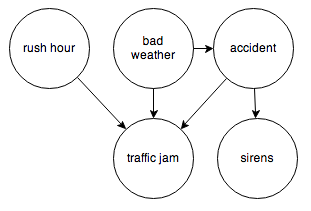
\includegraphics[width=0.5\textwidth]{trafficjam.png}
\caption{An example of a simple DAG \cite{traffic_jam}}
\end{figure}

Each arc represents a conditional probability relationship. Nodes in the graph are assumed to be conditionally independent of all nodes which are not its parents. For example, in figure \ref{dag1}: 

\begin{equation}
    \label{eq1}
    p(sirens | data) = p(sirens | accident)
\end{equation}

These conditional probabilities are abstract in the sense that they could be treated as either discrete or continuous. While much of the literature surrounding Bayesian Networks focuses on the discrete case, in the context of macroeconomic data we are generally dealing with continuous variables. This is possible as long as we are willing to make some assumptions about the nature of the conditional probability (as truly non-parametric estimation of continuous variables implies an intractably large search space). The most common assumption here (and fortunately the most natural economic one), is that the conditional distributions follow a multivariate normal distribution of the conditioning variables. This is implies the familiar form that conditional distributions are linear functions of conditioning variables with Gaussian errors, which is exactly the assumptions of simple, small-sample OLS. Such models are sometimes known as "Gaussian Bayesian Networks." For example:

\begin{equation}
    \label{eq2}
    sirens|data = sirens|accident = \alpha + \beta accident + \epsilon, \space \epsilon \sim N(0, \sigma^2)
\end{equation}

Therefore, this technique is "non-parametric" in the sense that we do not make any assumptions about which underlying relationships exist between variables (indeed, this is what we hope the model will tell us). However, we do make a parametric assumption about the conditional distributions.

\subsection{Estimation}

There are two fundamental problems to solve when estimating a DAG. The first is known as "Parameter Learning," and the other "Structure Learning." Given a DAG as in Figure \ref{dag1}, the first task is simply to estimate the parameters of the network, such as $\alpha$ and $\beta$ in Equation \ref{eq2}. This is usually done via maximum likelihood, however, other "score" functions are available such as the Bayesian Information Criterion (BIC) \cite{chen1998speaker}.

\begin{figure}
\centering
\label{dag2}
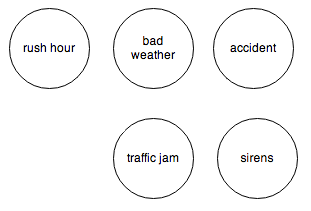
\includegraphics[width=0.5\textwidth]{trafficjam_unfit.png}
\caption{A DAG before structure learning}
\end{figure}

The second task, as demonstrated by Figure \ref{dag2} is that if we just start with some data it is not obvious which conditional probabilities to estimate in the first place. One way of achieving this is for the researcher to specify explicitly which conditional probabilities should be present in the graph, and simply fit the parameters of that graph. This however, is not what I am particularly interested in. If this is done the researcher has effectively specified a system of OLS equations to be estimated, probably based on some economic model that they already had in mind, and while this is then automatically encapsulated in a convenient, easily interpreted representation, it seems nothing of profound economic significance would have been achieved. 

The much more exciting avenue is to learn the structure of the graph from the data. One "brute force" method to solving this problem is to compute the posterior likelihood of every possible network, however, this number is super-exponential in the number of variables such that it becomes very computationally expensive, very quickly \cite{chickering1996learning}. As a response to this, many approximation techniques have been developed. These can be grouped into two categories: constraint-based and score-based structure learning algorithms \cite{spirtes1991algorithm} \cite{verma1991equivalence}. Constraint-based algorithms rely on the fact that changing the direction of an arc changes the conditional independences implied by the graph, the presence of which can be tested for from the data. Score-based methods as the name implies assign some score to every network based on its predictive accuracy and then use gradient-decent to identify the optimum network structure. In the application in this paper I have used the PC constraint-based algorithm \cite{spirtes2000causation} \cite{le2015parallelpc}.

Can this really work? Well in the right circumstances it indeed can! Consider the following simple example:

\begin{verbatim}
    library(bnlearn)
    library(parallel)
    library(combinat)
    # Fixes bug with bnlearn
    assignInNamespace("supported.clusters", 
                      c("cluster", "MPIcluster",  
                        "PVMcluster", "SOCKcluster"), 
                      "bnlearn")
    cl = makeCluster(4)
    ### Very simple example with confounding
    # Setup
    n <- 10000
    z <- rnorm(n)
    w <- rnorm(n)
    u <- rnorm(n, 0, 10)
    v <- rnorm(n, 0, 1)
    x <- 2*z + 2*w + u
    y <- 2*x + w + v
    # We have to introduce some asymmetry to make learning possible.
    data <- data.frame(z, w, u, v, x, y)
    names(data) <- c("z", "w", "u", "v", "x", "y")
    train <- data[1:floor(0.8*nrow(data)),]
    test <- data[(floor(0.8*nrow(data))+1):nrow(data),]
    
    # Structure Learning
    model <- pc.stable(train, cluster = cl, alpha=0.05)
    graphviz.plot(model)

    # Parameter Learning
    model <- bn.fit(model, train)
    model
\end{verbatim}

\begin{figure}
\centering
\label{dag4}
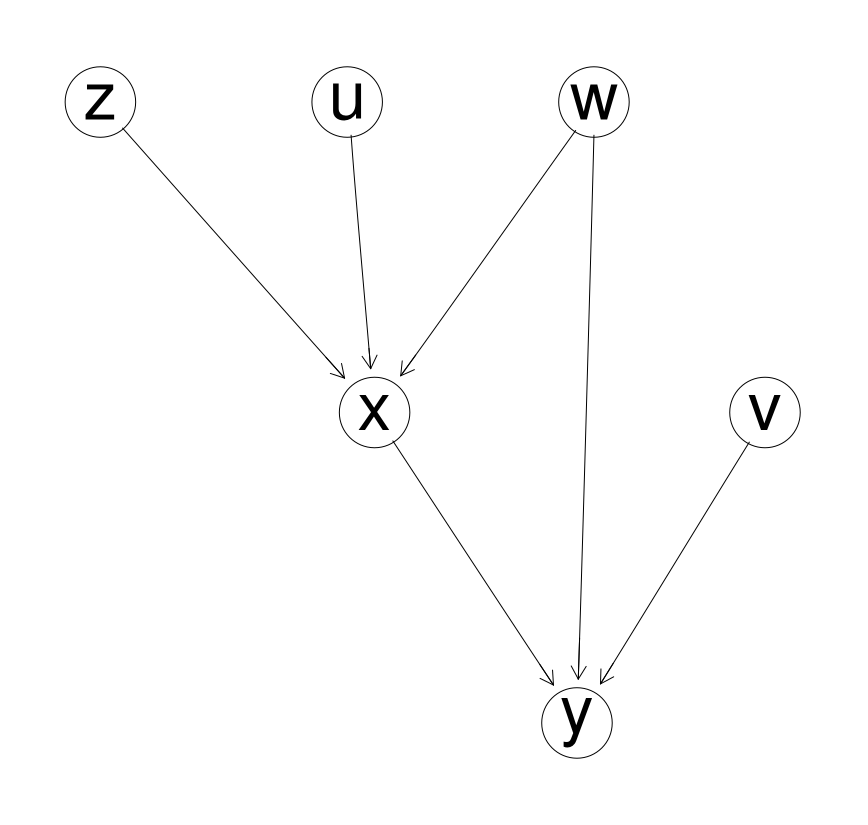
\includegraphics[width=0.5\textwidth]{simple_example.png}
\caption{DAG learned in simple example}
\end{figure}

This code results in\footnote{If you were to try this, it might in fact not, because the random number generation and structure learning algorithms are non-deterministic.} the DAG shown in \ref{dag4}, which is exactly a correct model of the underlying DGP. Once the structure is learned, parameter learning is relatively easy. Here are the parameters that are produced:

\begin{verbatim}
      Bayesian network parameters
    
      Parameters of node z (Gaussian distribution)
    
    Conditional density: z
    Coefficients:
     (Intercept)  
    -0.004053329  
    Standard deviation of the residuals: 1.011733 
    
      Parameters of node w (Gaussian distribution)
    
    Conditional density: w
    Coefficients:
    (Intercept)  
    -0.02413118  
    Standard deviation of the residuals: 1.007208 
    
      Parameters of node u (Gaussian distribution)
    
    Conditional density: u
    Coefficients:
    (Intercept)  
    -0.08107861  
    Standard deviation of the residuals: 10.05893 
    
      Parameters of node v (Gaussian distribution)
    
    Conditional density: v
    Coefficients:
     (Intercept)  
    -0.004851301  
    Standard deviation of the residuals: 1.00607 
    
      Parameters of node x (Gaussian distribution)
    
    Conditional density: x | z + w + u
    Coefficients:
     (Intercept)             z             w             u  
    4.543038e-16  2.000000e+00  2.000000e+00  1.000000e+00  
    Standard deviation of the residuals: 5.040424e-15 
    
      Parameters of node y (Gaussian distribution)
    
    Conditional density: y | w + v + x
    Coefficients:
     (Intercept)             w             v             x  
    1.191616e-16  1.000000e+00  1.000000e+00  2.000000e+00  
    Standard deviation of the residuals: 6.434891e-15 
\end{verbatim}

The parameters are exactly correct. Obviously, this is a very trivial example. Simple OLS would also identify everything here perfectly. This is simply meant to show that structure and parameter learning are possible in the right setting.

I believe that structure learning is the greatest contribution of the Bayesian Network framework. Many of the topics in this paper should seem quite familiar to any econometrician because they are fundamentally the same as some basic econometric concepts, although perhaps expressed through different language. However, the novel benefit of using this method is that we are effectively able to estimate a structural model directly from the data, without first having to specify which relationships we believe should be present.

\subsection{Inference}
Once a DAG has been fit to some data, there are a number of useful inferences that can be made. 

Firstly, nodes in the DAG which have no parents are known as "root-nodes." In the context of an economic application we can interpret these as the exogenous variables of the model. Since there is nothing to condition them on set $\beta$ to 0 in Equation \ref{eq2}, and observe that any such variables are implicitly modelled as i.i.d. Gaussian shocks. In particular, in the application I will seek to identify the exogenous variables in a macroeconomic simulation as the root-nodes of the associated Bayesian Network.

Furthermore, Bayesian Networks can be used to estimate counterfactual outcomes, using what Pearl \cite{pearl2009causality} describes as "do-calculus." Since the DAG specifies conditional independences, it is possible to (exogenously) modify one or more values of input data to some alternative value, and then calculate the predicted values of some other outcomes in the model in order to observe what the model predicts "would have happened" in that scenario. Furthermore, we could predict what might happen in any fabricated future scenario, as long as all of the exogenous variables are given some value. Assuming the DAG is the correct model of the true DGP (in fact, the conditions are weaker than this, see "faithfulness" in \cite{pearl2009causality}), then the effect on outcomes of such interventions can be given causal interpretations. 

For example, consider Figure \ref{dag3}. Suppose for simplicity that all of the variables are binary (1 in the presence of the event, 0 otherwise). On the LHS of the diagram we have the model for observed values of all of the variables. On the RHS we intervene on "accident." Notice that doing so breaks the link between "bad weather" and "accident." We can now estimate the causal treatment effect of an accident on the probability of a traffic jam given some values of "bad weather" and "rush hour" (in other words, all else equal) according to the equation:

\begin{equation}
    \label{eq3}
    p(tj | bw = \bar{bw}, rh = \bar{rh}, do(a=1)) - p(tj | bw = \bar{bw}, rh = \bar{rh}, do(a=0))
\end{equation}


\begin{figure}
\centering
\label{dag3}
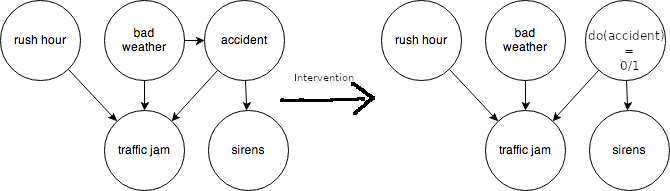
\includegraphics[width=\textwidth]{trafficjam_intervention.png}
\caption{An example of intervention}
\end{figure}

In addition, there are other kinds of possible prediction exercises that we may be interested in with some economic interpretation. Since the model defines every endogenous variable as a (linear) function of the exogenous shocks it can be interpreted similarly to a "rational expectations solution" from macroeconomics. Therefore, we might compute impulse response functions (IRFs) for each endogenous variable in the model to one or more shocks.

\subsection{Limitations}

Before continuing on to my application I would like to point out some of the limitations both of this methodology, and of my own knowledge in order to give some idea of the pitfalls that might be encountered during the course of this research. 

The concept of a DAG, while a powerful tool, is not a perfect model for all data. The strongest assumption is that it is directed. In many economic applications, while we may believe that some variables are truly exogenous such that they must be causes of movement in endogenous variables and not the other way around, we usually also assume that some or all of the endogenous variables are determined in general equilibrium, that is to say there is not necessarily a directionality to every relationship between endogenous variables. This problem while important, is probably not a show stopper. Structure learning algorithms do not force a direction onto every arc, it is merely optional. When some arcs in the model are undirected it is known as a, "hybrid network." However, it may be difficult to estimate the parameters of hybrid networks, because in the case of a bidirectional relationship it is unclear what parameters the model should specify. This is the problem of simultaneity that we are familiar with in econometrics. However, we can probably get around this by modelling the joint distribution of the simultaneous variables, conditional on the parent nodes.

Upon first being exposed to these ideas many are critical whether it is even conceptually possible to make such causal inferences directly from data. The section on structure learning gives some very brief overview of how we try to go about practically solving this problem. As far as the conceptual problem is concerned I do not yet understand it well enough myself to make a compelling argument. It is clear that going forward with this research will require me to do much deeper reading about the justification of direct structural learning. However, being the pragmatist that I am, it is for this reason that I have chosen to perform some direct applications in order to demonstrate simply whether or not such a strategy is likely to bear fruit, regardless of the strength of its theoretical underpinnings. The results so far have not been perfect, but I believe it has been successful enough to warrant further investigation into this topic.

\section{Application}

\subsection{Data}

In order to demonstrate the capability of the Bayesian Network method empirically I have chosen to use simulated data from macroeconomic models. This is not completely arbitrary; I envisage using simulated along with real macroeconomic data in my actual thesis. There are a few key reasons why I have chosen to work with this data. Firstly, since the model which simulates the data is known it is possible to say whether the structure learning has succeeded in identifying the underlying relationships in the data. In other words, since the true DGP is known it is possible to infer whether the estimated DAG faithfully represents the underlying DGP. Secondly, in the context of a log-linearized macroeconomic model the parametric assumptions (that conditional distributions are linear with Gaussian errors) is in fact correct. Finally, and more personally, given the choice of an application in microeconomics or macroeconomics I prefer one in macroeconomics because that is what I find more interesting.

\subsection{Methodology}

In order to collect this data I have found a repository of Dynare code for simulating many well-known macroeconomic DSGE models \cite{pfeifer2020}. I then modified this code slightly such that the output would be a data file containing simulated values of i.i.d. shocks and endogenous variables. I then load this data into R, and using the "bnlearn" package \cite{scutari2020}, I fit a Bayesian Network, using the PC algorithm to learn the structure because it is the default, and seemed to perform best in my short experimentation. Finally, I estimate the parameters of the model using maximum likelihood. Once the model is fit I perform a few experiments to evaluate the model performance.

\subsection{Results}

At this point, I would like to note that I have tried to perform this analysis for a few models, and it does not seem to work well for all of them. In the next section I will discuss the results for a baseline RBC model for which the results have been rather promising. On the other hand, I have attempted to model the medium-scale New Keynesian model from \cite{smets2007shocks}, without much success. In this model there are a large number of variables, many of which seem to actually measure the same thing, so it is hardly surprising that the algorithm becomes confused. Therefore, I would not like to completely write this one off. On the contrary, I bring this up to point out that while this is potentially a very useful modelling technique it is not a "magic bullet." Some assumptions on input data will be required. It is likely that some substantial part of my thesis will be dedicated to understanding in what situations Bayesian Networks work well, as well as what assumptions might be needed to guarantee that a faithful DAG can/will be found.

The data that I have used in this comes from a relatively detailed RBC model with a good number of variables to study. Table \ref{tab1} gives a summary of the variables in the data. In this model "z" and "g" are exogenous and both follow an AR(1) process. I exclude the actual period t shock to these variable (since this in unobservable in reality anyway) and include only their levels\footnote{However, I will note that this choice is not innocuous in the sense that it changes the results non-trivially. Indeed, the Bayesian Networks seem to fit better (despite the nature of the parametric assumptions) if the exogenous variables have some persistence, rather than being strictly i.i.d.}. Capital is also exogenous in period t because it is chosen (endogenously) in period t-1. For the sake of space, I will forego any further discussion of the relationships between endogenous variables, stating simply that these are of the standard RBC nature.

\begin{table}
\centering
\begin{tabular}{|l|l|l|}
  \hline
  Symbol & Name & Exogenous? \\
  \hline
  g & government spending & yes \\
  z & technology process & yes \\
  k & capital & yes \\
  w & wage rate & no \\
  r & return to capital & no \\
  y & output & no \\
  c & consumption & no \\
  l & hours worked & no \\
  invest & investment & no \\ \cline{2-2}
  \hline
\end{tabular}
\caption{Description of Variables}
\label{tab1}
\end{table}

\begin{figure}
\centering
\label{rbcdag}
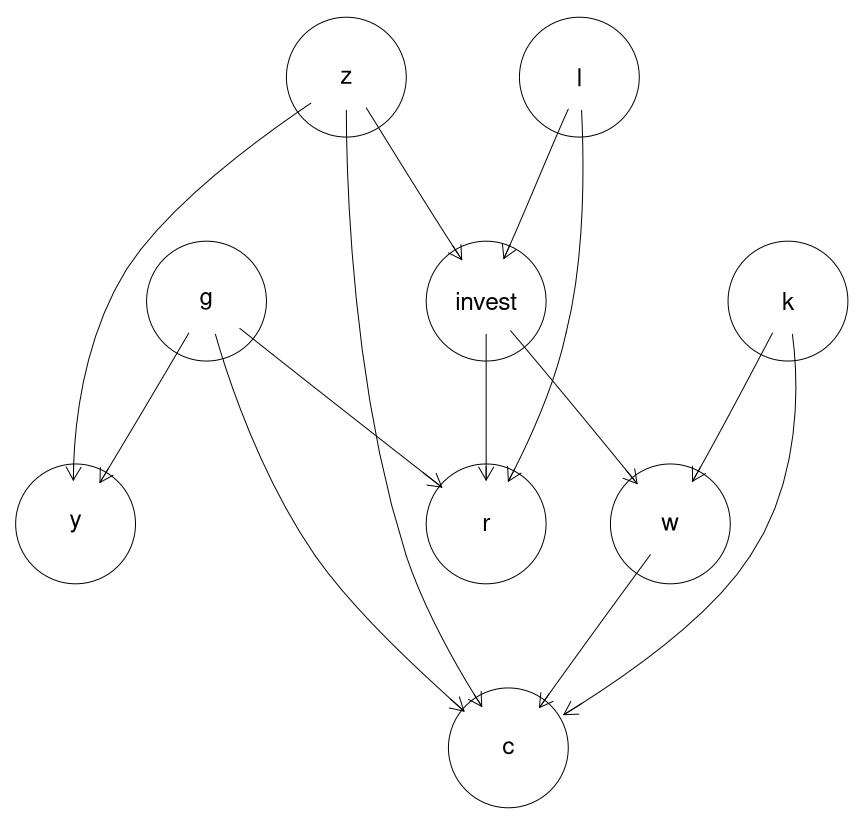
\includegraphics[width=\textwidth, height=0.4\textheight, keepaspectratio]{rbc_baseline_model.png}
\caption{Structure of DAG fit to RBC data}
\end{figure}

\begin{figure}
\centering
\label{rbcirf}
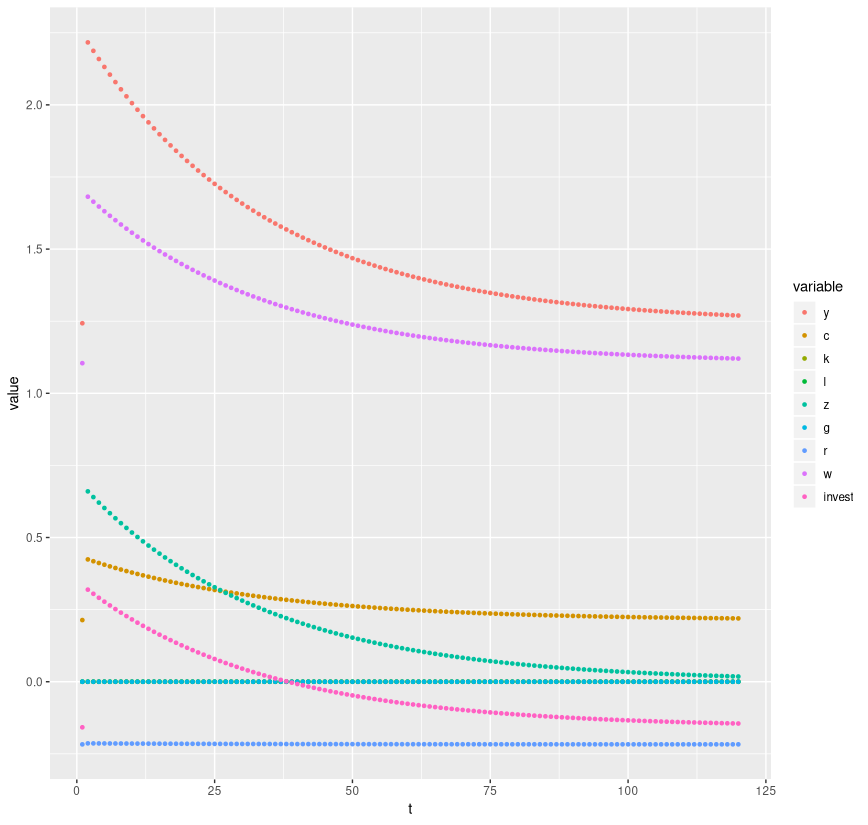
\includegraphics[width=\textwidth, height=0.4\textheight, keepaspectratio]{rbc_irf_ar1.png}
\caption{IRFs to technology shock predicted by model}
\end{figure}

Figure \ref{rbcdag} shows the structure of the DAG that was fit to the RBC data, with a sample size of 200. Here we note that structure learning successfully identified the three exogenous variables in the model as root nodes. However, it also identifies hours worked as a root node, even though this variable is not exogenous. Since the graph is fully directed we are able to fit parameters to the model in order to perform predictions. For example, we can perform pure prediction on output. In the spirit of best practice for machine learning we split the data into training and test data sets, and use only the training data to fit the parameters of the model. When doing this we find that the accuracy of predicting any endogenous variable in the test data is extremely high ($R^2 \approx 1$), although it should be noted that the variables are perfectly co-linear, so this prediction exercise is not exactly challenging. 

A more interesting exercise is to compute IRFs for the endogenous variables. Figure \ref{rbcirf} shows the result of computing IRFs for endogenous variables to a positive $AR(1)$ technology shock of one standard deviation. This is calculated by setting the value of "z" to decay by $\alpha_z$ every period from an initial value of 1 standard deviation, setting the other shocks to 0, and then calculating the predicted values for all of the endogenous variables\footnote{Note that "l" is excluded because the model thinks it is exogenous.}. Therefore, each period we are calculating the estimated treatment effect on every endogenous variable of an exogenous technology shock, all else equal. Qualitatively, the results are much what we would expect to see from an RBC model. 

\section{(Sketch) Research Plan}
There are a few ways that I can see taking this research, given the strengths and weaknesses which I have identified so far. Probably the first thing I would like to look at is trying to identify under what conditions structure and parameter learning algorithms are likely to succeed in finding an accurate model for the data. This will involve further investigation into the assumptions required by Bayesian Networks, and how they translate in the context of economics. If it proves to be infeasible to do this with macroeconomic simulations because the assumptions are unlikely to be satisfied, I might go looking for examples of economic data which are more likely to satisfy these conditions. Alternatively, if I find that Bayesian Networks really are a good model for this data, but that the structure learning algorithms seem to fail anyway, I might continue by manually specifying the structure before fitting parameters. While I think this would be less interesting (because I have already argued that structure learning is probably the most exiting thing about Bayesian Networks), I still think this research would be worth pursuing. Finally, regardless of what form the final thesis takes I really want to take it to real data. I have decided to start with simulated data because I think it is an excellent tool to illustrate how and when these tools can be useful. However, if I can succeed in making a strong argument that these models can learn effectively under some conditions, then obviously the most interesting thing will be to take it to real data and see what sort of implications the model gives us.  

\printbibliography

\end{document}
